\chapter{User Guide}
This user guide provides a overview of FuxCP, covering its installation process, usage within OpenMusic, and a description of the costs displayed in the interface. While FuxCP is designed to be compatible with all platforms, it relies on GiL, which currently works only on MacOS and Linux. Unfortunately, GiL does not support Windows due to compatibility issues between the 32-bit Lisp license used by OpenMusic and the 64-bit Gecode Windows version. Although it is technically possible to obtain a 32-bit version of Gecode for Windows, it is not recommended. 

\section{Installing FuxCP}
\subsection{Prerequisites}
To use FuxCP, it is necessary to download and install the following tools:
\begin{itemize}
    \item Gecode : \url{https://www.gecode.org/download.html/}
    \item OpenMusic : \url{https://openmusic-project.github.io/openmusic/}
\end{itemize}

And download the following libraries:
\begin{itemize}
    \item GiL : \url{https://github.com/sprockeelsd/GiLv2.0/}
    \item FuxCP : \url{https://github.com/sprockeelsd/Melodizer/}
\end{itemize}
On the latest GitHub there are other tools available such as Melodizer and Melodizer2.0. For the purposes of this guide, only the FuxCP folder will be needed.

\subsection{Loading FuxCP in OpenMusic}
In order to use the above libraries, OpenMusic must be running. When opening any workspace, locate the toolbar at the top of the interface. Click on the "Windows" button, highlighted in the figure \ref{fig:library}, and select "Library" from the drop-down menu. This will bring up a new window. From the toolbar of this window, select 'File' and then 'Add Remote Library'. Navigate through your file system to find the path where the previously downloaded FuxCP and GiL libraries are stored. Once located, the libraries should appear under the "Libraries" folder in the "Library" window, as shown in Figure \ref{fig:load}. Right click on "fuxcp" and select "Load Library". If no errors occur, the setup is complete.

However, if an error arises, it may be a linking issue with the Gecode library. For MacOS users, a script can be used from the \texttt{c++} folder of the GiL library. Edit the path to Gecode inside the script to match your system's configuration. Linux users should add the Gecode library to the \texttt{LD\_LIBRARY\_PATH} variable. Go to the \texttt{/etc/ld.so.conf.d} folder and create a new \texttt{.conf} file if one does not already exist. In this file, paste the full path to the Gecode library, save it, and run \texttt{sudo ldconfig} to update the system with the new library. Don't forget to restart OpenMusic and don't stop believing. Following these steps should ensure the proper utilization of FuxCP.

\begin{figure}[h]
    \centering
    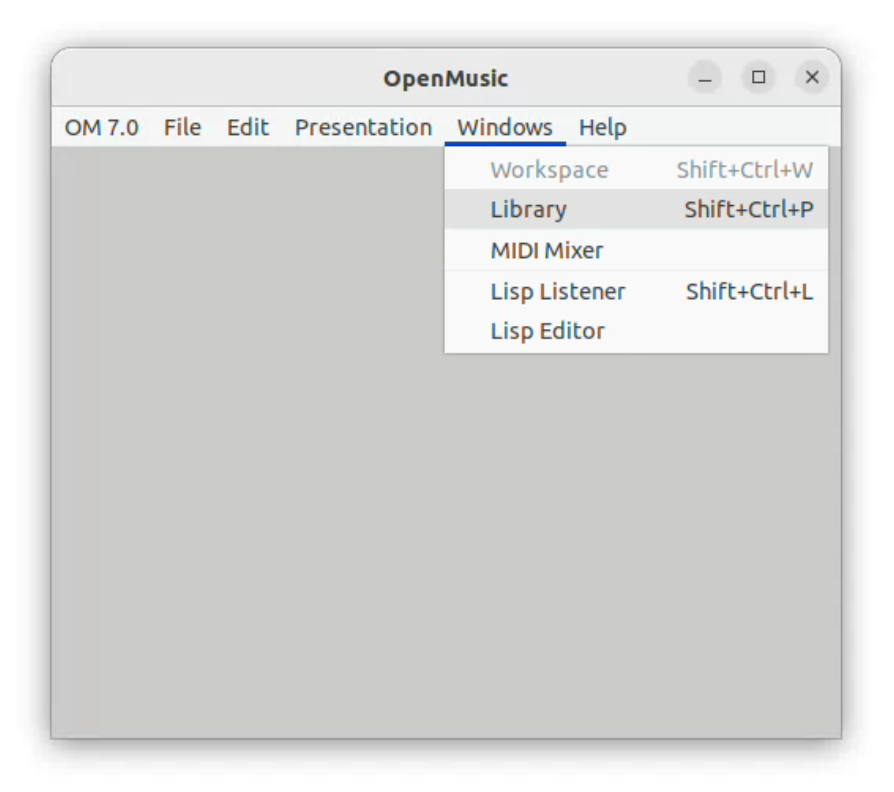
\includegraphics[height=2.6in]{Images/openmusic_library.png}
    \caption{Opening the "Library" window in OpenMusic.}
    \label{fig:library}
\end{figure}
\begin{figure}[h]
    \centering
    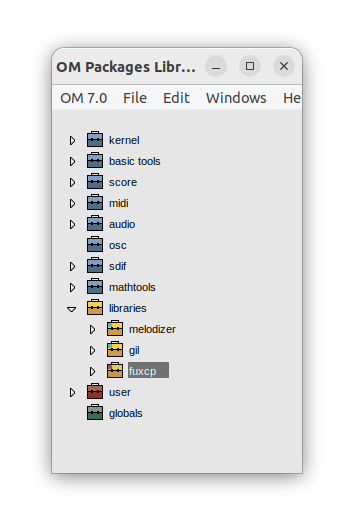
\includegraphics[height=2.6in]{Images/openmusic_load.png}
    \caption{Loading the "fuxcp" library in OpenMusic.}
    \label{fig:load}
\end{figure}

\section{Using FuxCP in OpenMusic}
It is straightforward to use FuxCP in OpenMusic. There is a single block comprising the entire graphical interface of the tool. This block or class is called \texttt{cp-params}. To load it, it is possible to type \texttt{fuxcp::cp-params} in a new patch entry; or load the block of the class by loading "cp-params" from the drop-down menu by right-clicking in the patch ($Classes\to Libraries\to FuxCP\to Solver\to CP-PARAMS$). Alternatively, you can just double-click anywhere in the patch, type "fuxcp::cp-params" and press Enter. This also works for "poly", "voice" and "x-append".

Once this block has appeared, all you have to do is bind an OM voice object, representing the \cfcomma to the second argument of \texttt{cp-params} as shown in figure \ref{fig:om_ext_interface_mod}. Don't forget to block the input voice object and evaluate \texttt{cp-params} so it can detect the new input. Now \texttt{cp-params} can be blocked too. From now on, you could directly use the interface and generate counterpoints using the tool. If you want to retrieve the voice object containing the counterpoint generated by the tool, just bind the third argument on the output side to a voice object. Once bound, it is then possible to evaluate the voice object so that it updates.

If you want to get the whole composition in one object, you have to do some fiddling with OpenMusic. The simplest way to do this is shown in Figure \ref{fig:om_ext_interface_mod}, and works as follows: get the POLY object returned by CP-PARAMS on its third output, split this object in two (the two voices), then get the \cfs, which is the second output of CP-PARAMS, and put all the voices back together in the desired order using x-append functions. 

\begin{figure}[h]
    \centering
    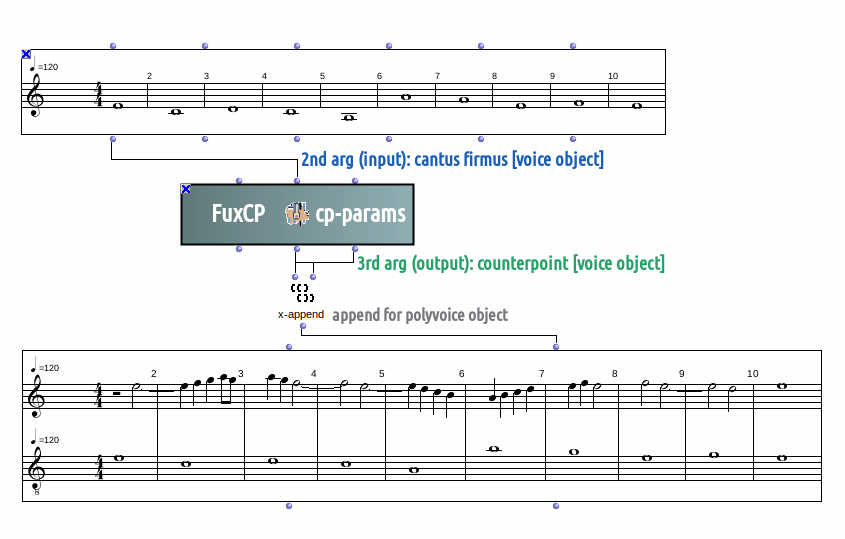
\includegraphics[width=5.2in]{Images/om_ext_interface_mod.png}
    \caption{View of a patch using \texttt{fuxcp::cp-params} in OpenMusic.}
    \label{fig:om_ext_interface_mod}
\end{figure}

But how do you use the interface? Simply double-click on the block to bring it up. The interface is sorted from left to right, so the preferences are divided into three different categories: "Preferences for Melodic Intervals of\dots", "General Preferences", "Species-Specific Preferences", "Solver Configuration", "Cost importance order of\dots", and, in the bottom right corner, "Solver Launcher" (see figure \ref{fig:om_int_interface}). Once you have chosen the preferences, the default ones representing the Fux style, you have to save the parameters ("Save Config") in order to start the search for a solution ("Next Solution"). This search may take a fraction of a second, or it may take tens of minutes if the parameters chosen make the search difficult. If the search takes too long, you can always stop it by clicking on "Stop". You can then either change the settings in some way (often by changing the voice range).

The parameters are described in the next section. As far as the "Cost importance order" panel is concerned, it works by setting an order of importance for the costs. This means that it will give priority to minimising the cost that has a high importance. The importance ranges from one to thirteen, with one being the most important. The option between Linear combination and Maximum minimisation is to know, in case two costs are set to have the same importance, how to combine the equally important costs at one level of the lexicographic search;

\paragraph{}
Pressing the "Next Solution" button will display the solution as a pop-up. What appears on the screen are the two counterpoints. The \cfs must be added manually as described at the beginning of this section. 


The other option is to press the "Best Solution" button. This will start an infinite search that will only stop when the best solution has been found (which can take hours). You can evaluate the output object at any time to see what the best result is so far, and this will not stop the search, so you can see how the solution improves step by step, and stop the search when it has produced something you are happy with.


Please note that the preferences do not affect the speed of finding the first solution. The first solution is the first valid solution and is not affected by the cost. Only the subsequent solutions can be affected by the preferences.

\begin{figure}[h]
    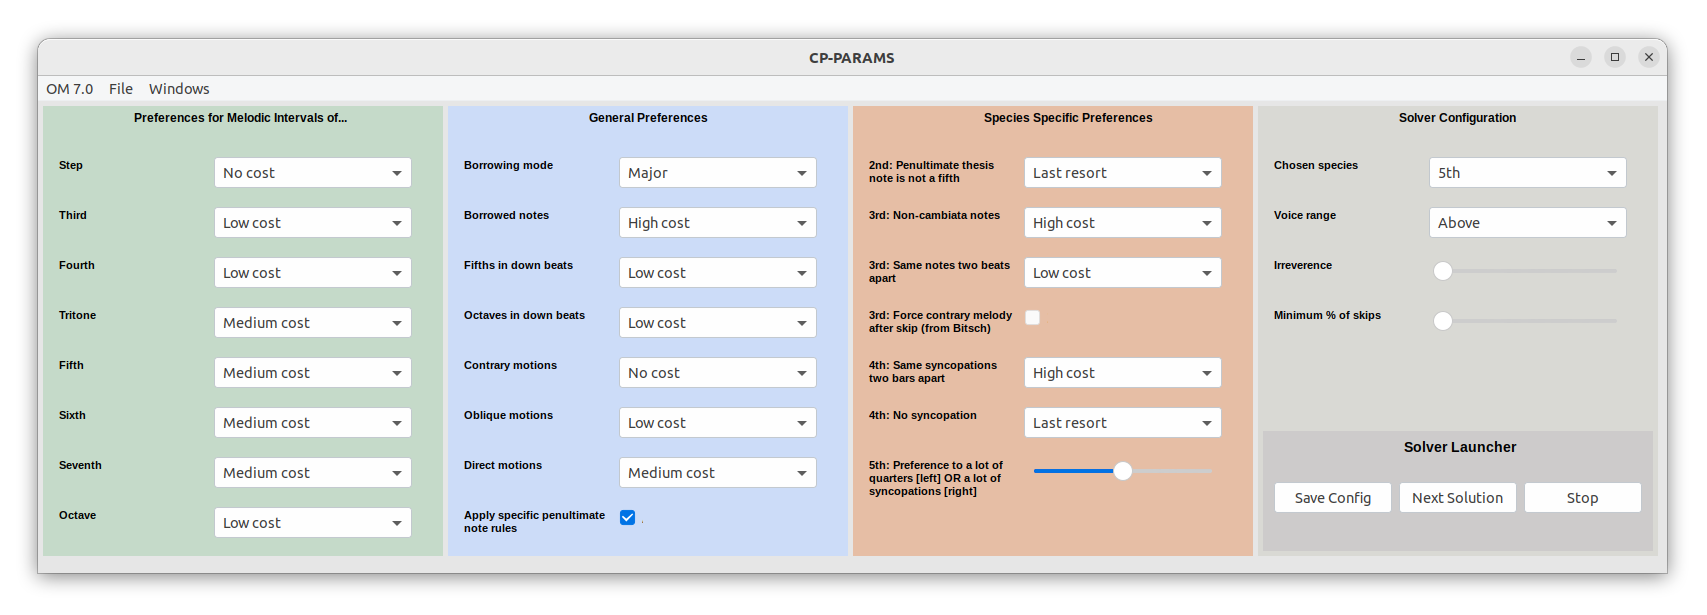
\includegraphics[width=1.2\textwidth, center]{Images/om_int_interface.png}
    \caption{User interface of the \texttt{fuxcp::cp-params} class in OpenMusic.}
    \label{fig:om_int_interface}
\end{figure}

\section{Interface Parameters Description} \label{appendix:interface-parameters-description}
Table \ref{tab:cp-params} describes all the parameters available in the interface. A low cost represents a high preference while a high cost represents a low preference.

\begin{table}[!h]
    \footnotesize
    \begin{adjustbox}{center}
        \begin{tabular}{|m{0.22\textwidth}|m{0.82\textwidth}|m{0.15\textwidth}<{\centering}|}
        \hline
        \multicolumn{1}{|c|}{\textbf{Name}} &
          \multicolumn{1}{c|}{\textbf{Description}} &
          \textbf{Default value} \\ \hline
        \cellcolor[HTML]{BCE08D}Step &
          Preference for melodic intervals of one step or less. &
          No cost \\ \hline
        \cellcolor[HTML]{BCE08D}Third &
          Preference for melodic third skips. &
          Low cost \\ \hline
        \cellcolor[HTML]{BCE08D}Fourth &
          Preference for melodic fourth leaps. &
          Low cost \\ \hline
        \cellcolor[HTML]{BCE08D}Tritone &
          Preference for melodic tritone leaps. &
          Forbidden \\ \hline
        \cellcolor[HTML]{BCE08D}Fifth &
          Preference for melodic fifth leaps. &
          Medium cost \\ \hline
        \cellcolor[HTML]{BCE08D}Sixth &
          Preference for melodic sixth leaps. &
          Medium cost \\ \hline
        \cellcolor[HTML]{BCE08D}Seventh &
          Preference for melodic seventh leaps. &
          Medium cost \\ \hline
        \cellcolor[HTML]{BCE08D}Octave &
          Preference for melodic octave leaps. &
          Low cost \\ \hline
        \hline
        \cellcolor[HTML]{C8D6FF}Apply specific penultimate note rules &
          Force all rules on the notes of the penultimate measure. This mainly refers to the penultimate note that must harmonically be either a major sixth or a minor third depending on whether the counterpoint is above or below. &
          Checked \\ \hline
        \cellcolor[HTML]{C8D6FF}Borrowing mode &
          Type of scale from which notes can be borrowed to generate counterpoint. The first note of the \cfs determines the tonic of this scale. Applies everywhere except the penultimate bar. &
          Major \\ \hline
        \cellcolor[HTML]{C8D6FF}Borrowed notes &
          Preference for borrowed notes outside the diatonic scale. These notes are defined by the "Borrowing mode" parameter. &
          High cost \\ \hline
        \cellcolor[HTML]{C8D6FF}Fifths in down beats &
          Preference to have harmonic fifths on the first beat of a bar. &
          Low cost \\ \hline
        \cellcolor[HTML]{C8D6FF}Octaves in down beats &
          Preference to have harmonic octaves on the first beat of a bar. &
          Low cost \\ \hline
        \cellcolor[HTML]{C8D6FF}Contrary motions &
          Preference to have, between two bars, one voice rising while the other is falling. &
          No cost \\ \hline
        \cellcolor[HTML]{C8D6FF}Oblique motions &
          Preference to have, between two bars, one static voice while the other is moving. &
          Low cost \\ \hline
        \cellcolor[HTML]{C8D6FF}Direct motions &
          Preference to have, between two bars, the two voices going in the same direction. &
          Medium cost \\ \hline
        \cellcolor[HTML]{C8D6FF}Successive perfect consonances &
          Preference to have as few successive perfect consonances as possible. &
          Medium cost \\ \hline
        \hline
        \cellcolor[HTML]{FFCE93}2nd: Penultimate thesis note is not a fifth &
          Preference for the first note of the penultimate bar to be something other than a harmonic fifth &
          Last resort \\ \hline
        \cellcolor[HTML]{FFCE93}3rd: Non-cambiata notes &
          Preference for the second quarter note of a bar to be a consonance already surrounded by two consonances. &
          High cost \\ \hline
        \cellcolor[HTML]{FFCE93}3rd: Same notes two beats apart &
          Preference to have the same quarter notes two beats apart. A high cost allows to avoid a certain monotony. &
          Low cost \\ \hline
        \cellcolor[HTML]{FFCE93}3rd: Force joint contrary melody after skip &
          Force that a melodic skip or leap is followed by a melodic step in the opposite direction. &
          Unchecked \\ \hline
        \cellcolor[HTML]{FFCE93}4th: Same syncopations two bars apart &
          Preference to have the same half notes two bars apart. A high cost allows to avoid a certain monotony. &
          High cost \\ \hline
        \cellcolor[HTML]{FFCE93}4th: No syncopation &
          Preference to have distinct half notes instead of syncopations. &
          Last resort \\ \hline
        \cellcolor[HTML]{FFCE93}5th: Preferences to a lot of quarters or a lot of syncopations &
          Determines the minimum percentage of quarter notes (to the left) and syncopations (to the right) in the fifth species. Pushing the slider all the way to one side is not recommended. &
          <center> \\ \hline
        \hline
        \cellcolor[HTML]{EFEFEF}Chosen species &
          Determines the type of counterpoint that the tool will generate. From whole notes to syncopations, passing through quarter notes. The fifth species uses the rules and preferences of all other species. &
          1st \\ \hline
        \cellcolor[HTML]{EFEFEF}Voice range &
          Determines around which pitch the counterpoint will be generated depending on the pitch of the first note of the \cfdot &
          Above and very far above \\ \hline
        \cellcolor[HTML]{EFEFEF}Minimum \% of skips &
          Determines, depending on the counterpoint size, the percentage of melodic intervals larger than one step. &
          0\% \\ \hline
        \cellcolor[HTML]{D1D1D1}Save Config &
          Saves all established preferences and allows you to start a new search for this configuration later. &
          - \\ \hline
        \cellcolor[HTML]{D1D1D1}Next Solution &
          Starts or continues searching for the previously saved configuration. Displays a new window with the solution when it is found. Displays an error message if no other solution can be found. &
          - \\ \hline
        \cellcolor[HTML]{D1D1D1}Stop &
          Pause the search. It may take up to 5 seconds. &
          - \\ \hline
        \end{tabular}
    \end{adjustbox}
    \caption{Description of the parameters of \texttt{fuxcp::cp-params}.}
    \label{tab:cp-params}
\end{table}

